\documentclass[a4paper]{article}
\usepackage[english]{babel}
\usepackage[utf8]{inputenc}
\usepackage{graphicx}

\title{A News System Implementation \\ C++ Programming, EDA031}

\author{Erik Hedblom, [tpi11ehe]
\and Tobias Landelius, [ael10tla]
\and Oskar Jermakowicz, [dat12oje]
\and Martin Larsson, [dat12mla]}



\date{\today}


\begin{document}
\maketitle

\newpage
\renewcommand{\contentsname}{Table of contents}
\tableofcontents
\newpage

\section{System description}
The application is a simple implementation of a news system where newsgroups and articles are stored on a server which communicates with clients that connect to it. The client is a Command Line Interface where users can execute commands to receive, edit or delete data on the server.

The implementation is divided into three packages as can be seen in Figure 1 below; \texttt{server}, \texttt{client} and \texttt{library}.

\begin{center}
% TODO: insert UML diagram
\textbf{Figure 1:} UML diagram of the system.
\end{center}

The purpose of both the server and the client will be further explained in detail in section 1.1 and 1.2 of this report. The purpose of the library is to handle the interaction between the server and the client...

\begin{center}
% TODO: insert UML sequence diagram
\textbf{Figure 2:} The interaction between server and client.
\end{center}

%% TODO %%
A detailed description of your system design, both for the server and the clients. Preferably
use UML diagrams to give an overview of the design. (It is not necessary that you list
attributes and methods in these diagrams.) You must also describe the classes, at least as
far as stating the responsibilities of each class.
Also give an overview of the dynamics of the server, i.e., trace an interaction between a
client and the server from the point that the server receives a command until it sends the
reply. UML sequence diagrams are good for this purpose.

\subsection{Server}

\subsection{Client}
In order to start a client, one has to run the following command on the command line in the directory of newsclient; \texttt{newsclient host-name port-number}. If the connection is successful, this will establish a connection with the server. The establishment of the connection is handled by the \texttt{NewsClient} constructor which creates a \texttt{Connection} object which will be used to communicate with the server.

Once a connection is established the \texttt{run()} method of \texttt{NewsClient} is run, and the user can now execute commands. All possible commands are explained if the user runs the command \texttt{help}, the printout of the \texttt{help} command can be seen in Appendix A.

The client parses each user input through regex to see whether the input is a valid command. This is done through \texttt{parse\_line(string)} which matches any valid commands and parameters and stores them in a vector. This vector is thereafter compared with the available commands in \texttt{handle\_command(string)}, and if it turns out the commands is valid, the corresponding method for that particular command is run in \texttt{NewsClient}. These methods simply call the different send commands in the \texttt{message} class in the \texttt{library} package. The start and end of the command is sent with the \texttt{send\_code(Connection, int)} method in \texttt{message}, where the int is the corresponding protocol definition from \texttt{protocol.h}. If the command has any parameters, these are sent with either \texttt{send\_int\_parameter(Connection, int)} or \texttt{send\_string\_parameter(Connection, string)}. Once the whole command has been sent to the server, the same method will check the servers response with \texttt{consume\_code(Connection, int)} (where int is a protocol definition) and \texttt{recv\_code(Connection)} in \texttt{message} and print the servers response to the user.


\section{Conclusion}

%% TODO %%
Conclusions: requirements that you fulfill, problems that you haven’t succeeded in solving,
etc. If you have found that the system ought to have more features you should elaborate on
this. Any suggestions for improvements to the project are also welcome.

\section*{Appendix A}
\addcontentsline{toc}{section}{Appendix A}

\begin{center}
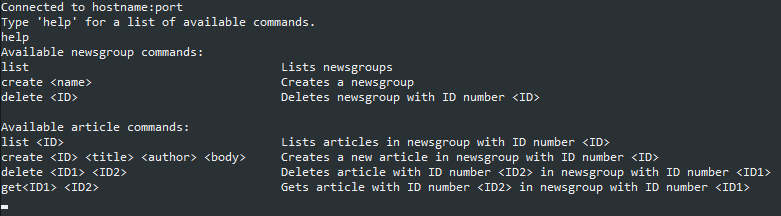
\includegraphics[scale=0.8]{help_text_appendix.png}
\textbf{Figure 3:} Available commands, shown when the \texttt{help} command is run.
\end{center}

\end{document}
